\section{SIFT Approach}
\label{sift}

Lowe's algorithm generates a set of keypoints along with keypoint descriptors.  These keypoints are selected by detecting areas of high curvature and contrast at all scales (Figure~\ref{sift_scales}), and then refined based on keypoint stability. The corresponding descriptors are then generated by calculating the gradient of the region, realigning the gradients to the largest relative gradient to provide local rotational invariance, and transforming the local gradients into a 128 bin feature vector (Figure~\ref{sift_kp_gradient}). The resulting array is resistant to changes in illumination and image distortion.

\begin{figure}[h]
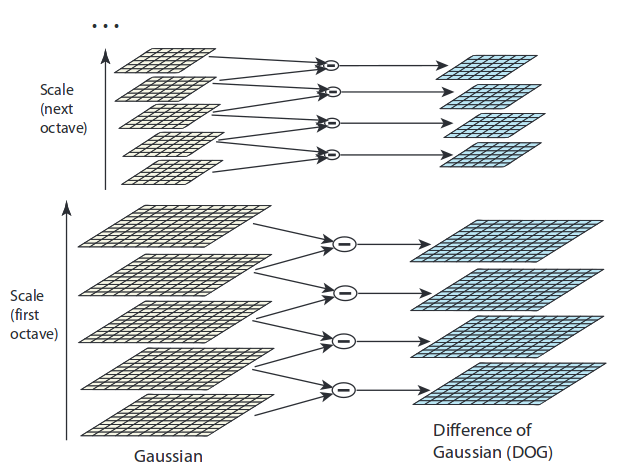
\includegraphics[scale=0.3]{dog_pyramid.png}
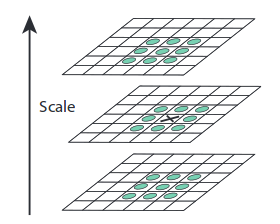
\includegraphics[scale=0.6]{pyramid_extrema.png}
\centering
\caption{Taken from Lowe \cite{SIFT}, an difference-of-Gaussian image pyramid is constructed to estimate the Laplacian at each level. At each pixel location, its neighbouring 26 pixels are checked for scale-space extrema as keypoint candidates.}
\label{sift_scales}
\end{figure}

These descriptors can then be used to match two keypoints together by comparing the Euclidean distance between any two pairs of keypoints. In his paper, Lowe suggests a method of 2-nearest neighbours matching where a correct match is determined by taking the ratio of the distance of the closest and the second closest matches. He proposes a ratio of 0.75 to be optimal, and in our testing we have found this to be accurate on our dataset of 215 training and 196 validation images (See Table~\ref{sift_ratios}). Due to the small size of this dataset, we opted to store our keypoints in-memory in an array and perform a brute-force match on all training data as opposed to storing in a k-d tree.

\begin{figure}[h]
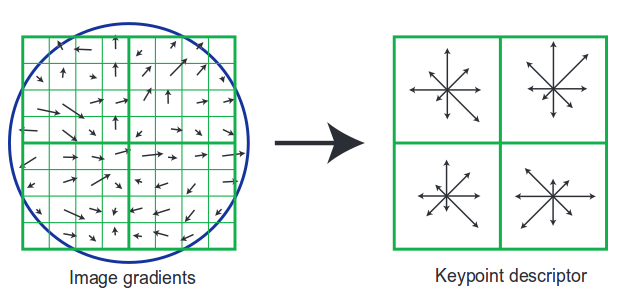
\includegraphics[scale=0.6]{keypoint_orientation.png}
\centering
\caption{Taken from Lowe \cite{SIFT}, the gradients of the keypoint region are divided into smaller windows. At each window, the gradients are rotated to align to the dominant gradient.}
\label{sift_kp_gradient}
\end{figure}

SIFT has a large limitation due to only working in one-dimensional color space, and consequently images need to be either converted to grayscale or run on only one color basis vector. By converting into grayscale, color-based depth and contrast information is lost and by extension, possible keypoint candidate locations. However, using only one color basis vector results in a similar predicament as the additional information encoded is not fully utilized. One possible workaround is to convert into HSV color space and to apply SIFT on the hue basis vector, as it retains color data at the cost of ``colorfulness." However, the drawback is that it takes a significant amount of time to convert from RGB color space to HSV, which detracts from our goal of a real-time gesture classifier.

\begin{figure}[h]
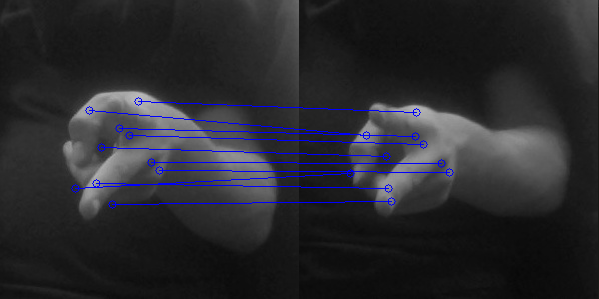
\includegraphics[scale=0.6]{kp_matching_left_test_right_train.png}
\centering
\caption{Visualization of matched SIFT keypoints. The image on the left is from the validation set, while the image on the right is from the training set.}
\label{sift_kp_matching}
\end{figure}